\documentclass[12pt]{article}
\usepackage[utf8]{inputenc}

\usepackage{lmodern}

\usepackage{enumitem}
\usepackage[margin=2cm]{geometry}

\usepackage{amsmath, amsfonts, amssymb}
\usepackage{graphicx}
%\usepackage{subfigure}
\usepackage{tikz}
\usepackage{pgfplots}
\usepackage{multicol}

\usepackage{comment}
\usepackage{url}
\usepackage{calc}
\usepackage{subcaption}
\usepackage[indent=0pt]{parskip}
\usepackage{animate}

\usepackage{array}
\usepackage{blkarray,booktabs, bigstrut}
\usepackage{bigints}

\pgfplotsset{compat=1.16}

% MATH commands
\newcommand{\ga}{\left\langle}
\newcommand{\da}{\right\rangle}
\newcommand{\oa}{\left\lbrace}
\newcommand{\fa}{\right\rbrace}
\newcommand{\oc}{\left[}
\newcommand{\fc}{\right]}
\newcommand{\op}{\left(}
\newcommand{\fp}{\right)}

\newcommand{\bi}{\mathbf{i}}
\newcommand{\bj}{\mathbf{j}}
\newcommand{\bk}{\mathbf{k}}
\newcommand{\bF}{\mathbf{F}}

\newcommand{\mR}{\mathbb{R}}

\newcommand{\ra}{\rightarrow}
\newcommand{\Ra}{\Rightarrow}

\newcommand{\sech}{\mathrm{sech}\,}
\newcommand{\csch}{\mathrm{csch}\,}
\newcommand{\curl}{\mathrm{curl}\,}
\newcommand{\dive}{\mathrm{div}\,}

\newcommand{\ve}{\varepsilon}
\newcommand{\spc}{\vspace*{0.5cm}}

\DeclareMathOperator{\Ran}{Ran}
\DeclareMathOperator{\Dom}{Dom}

\newcommand{\exo}[1]{\noindent\textcolor{red}{\fbox{\textbf{Problem {#1}}}\hrulefill}\\\\ }
\newcommand{\qu}[4]{\noindent\textcolor{#4}{\fbox{\textbf{Section {#1} | Problem {#2}}} \hrulefill{{\fbox{\textbf{{#3} Points}}}}\\}}

\newcommand{\semester}{Fall 2023}

\newcommand{\CVup}{%
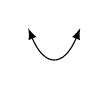
\begin{tikzpicture}
\draw[black, <->, >=latex] (-0.33, 0.5) .. controls (-0.125, 0) and (0.125, 0) .. (0.33, 0.5);
\end{tikzpicture}}

\newcommand{\CVupInc}{%
\begin{tikzpicture}
\draw[black, ->, >=latex] (0,0) .. controls (0.2, 0) and (0.4, 0.2) .. (0.5, 0.5);
\end{tikzpicture}}

\newcommand{\CVupDec}{%
\begin{tikzpicture}[rotate=270]
\draw[black, ->, >=latex] (0,0) .. controls (0.2, 0) and (0.4, 0.2) .. (0.5, 0.5);
\end{tikzpicture}}

\newcommand{\CVdown}{%
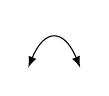
\begin{tikzpicture}
\draw[black, <->, >=latex] (-0.33, -0.5) .. controls (-0.125, 0) and (0.125, 0) .. (0.33, -0.5);
\end{tikzpicture}}

\newcommand{\CVdownInc}{%
\begin{tikzpicture}
\draw[black, ->, >=latex] (-0.5, -0.5) .. controls (-0.5, -0.3) and (-0.5, -0.1) .. (0,0);
\end{tikzpicture}}

\newcommand{\CVdownDec}{%
\begin{tikzpicture}[rotate=-90]
\draw[black, ->, >=latex] (-0.5, -0.5) .. controls (-0.5, -0.3) and (-0.5, -0.1) .. (0,0);
\end{tikzpicture}}

\begin{document}
	\noindent \hrulefill \\
	MATH-244 \semester \hfill Practice Problems Solutions\\
	Section 16.4 \hfill Pierre-Olivier Paris{\'e} \\\vspace*{-1cm}
	
	\noindent\hrulefill
	
	\spc	

	\exo{6}
	\\
	We have $P(x, y) = x^2 + y^2$ and $Q(x, y) = x^2 - y^2$. By Green's Theorem, we have
		\begin{align*}
		\oint (x^2 + y^2 ) dx + (x^2 - y^2 ) dy = \iint_D Q_x - P_y \, dA .
		\end{align*}
		
	The domain $D$ is the triangle with vertices $(0, 0)$, $(2, 1)$, and $(0, 1)$. The positive orientation is a parametrization that passes to all the points in the following order: $(0, 0)$ to $(2, 1)$ to $(0, 1)$ and then coming back to $(0, 0)$. We can write
		\begin{align*}
		D = \{ (x, y) \, : \, 0 \leq x \leq 2 , x/2 \leq y \leq 1 \} .
		\end{align*}
	Thus, 
		\begin{align*}
		\iint_D 2x - 2y \, dA = \int_0^1 \int_{x/2}^1 2x - 2y \, dy dx = 0 .
		\end{align*}
	So the line integral is zero.
	
	\spc
	
	\exo{12}
	\\
	We see that $P(x, y) = e^{-x} + y^2$ and $Q(x, y) = e^{-y} + x^2$ and so 
		\begin{align*}
		Q_x - P_y = 2x - 2y .
		\end{align*}
	We want to compute
		\begin{align*}
		\int_C \vec{F} \cdot d \vec{r} = \int_C e^{-x} + y^2 \, dx + e^{-y} + x^2 \, dy .
		\end{align*}
	The curve (in red) and the domain (in green) bounded by the curve is represented below.
		\begin{figure}[ht]
		\centering
		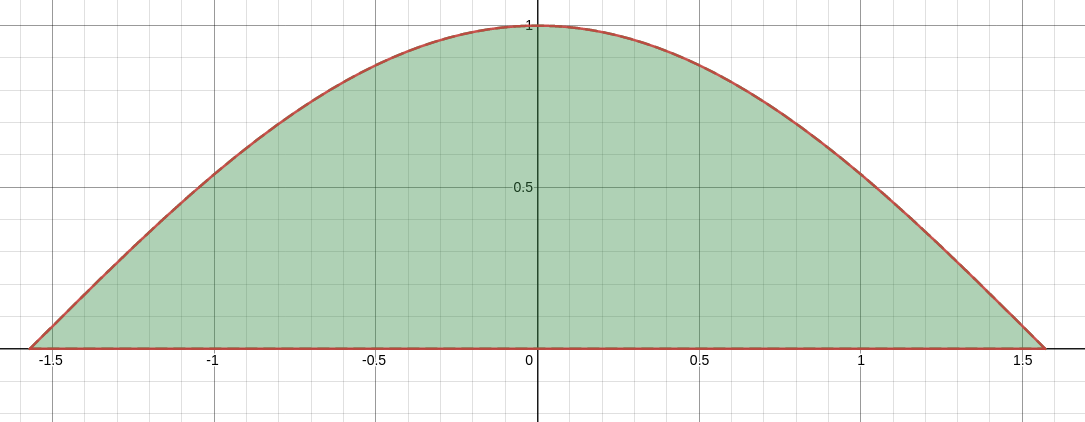
\includegraphics[scale=0.3]{picture1.png}
		\end{figure}
	Taking the counterclockwise orientation on the curve, we can write
		\begin{align*}
		\int_C e^{-x} + y^2 \, dx + e^{-y} + x^2 \, dy = \oint_C e^{-x} + y^2 \, dx + e^{-y} + x^2 \, dy 
		\end{align*}
	and by Green's Theorem, we obtain
		\begin{align*}
		\oint_C e^{-x} + y^2 \, dx + e^{-y} + x^2 \, dy = \iint_D Q_x - P_y \, dA = \iint_D 2x - 2y \, dA .
		\end{align*}
	
	The description of $D$ is
		\begin{align*}
		D = \{ (x, y ) \, : \, -\pi/2 \leq x \leq \pi/2 , \, 0 \leq y \leq \cos x \} .
		\end{align*}
	So, we obtain
		\begin{align*}
		\iint_D 2x - 2y \, dA = \int_{-\pi/2}^{\pi/2} \int_0^{\cos x} 2x - 2y \, dy dx = \pi/2 .
		\end{align*}
		
	\spc
	
	\exo{18}
	\\
	Here is the path traced by the particle and the region $D$ enclosed by the curve $C$.
		\begin{figure}[ht]
		\centering
		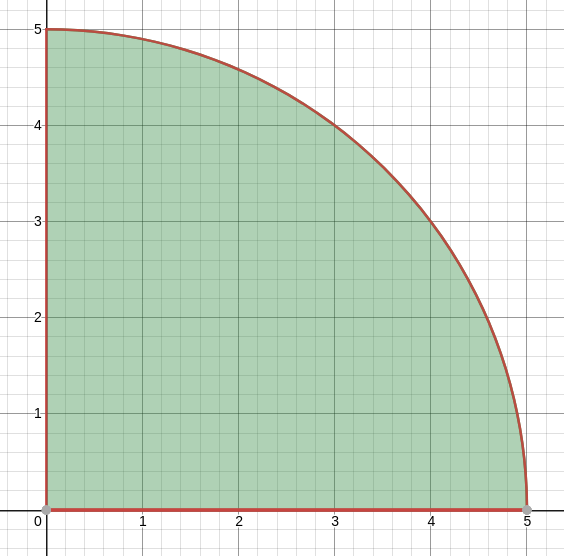
\includegraphics[scale=0.3]{picture2.png}
		\end{figure}
	The work is given by
		\begin{align*}
		W = \int_C \vec{F} \cdot d\vec{r} 
		\end{align*}
	where $\vec{F} (x, y) = \left\langle \sin x , \sin y + xy^2 + \frac{1}{3} x^3 \right\rangle$. Taking the counterclockwise orientation, we see from Green's Theorem that
		\begin{align*}
		W = \iint_D Q_x - P_y \, dA .
		\end{align*}
	
	We have
		\begin{align*}
		D = \{ (x, y) \, : \, 0 \leq x \leq 5 , \, 0 \leq y \leq \sqrt{25 - x^2} \},
		\end{align*}
	$Q_x = y^2 + x^2$ and $P_y = 0$, so
		\begin{align*}
		W = \int_0^5 \int_0^{\sqrt{25 - x^2}} x^2 + y^2 \, dy dx .
		\end{align*}
	We change to polar coordinates. We have
		\begin{align*}
		W = \int_0^5 \int_0^{\pi/2} r^2 \, d\theta dr = \frac{125 \pi}{6} \approx 65.4498 .
		\end{align*}


\end{document}